\documentclass[10pt,letterpaper]{article}
\usepackage{geometry}
\geometry{margin=1in}
\usepackage{graphicx}
\usepackage{booktabs}   
\usepackage{xltabular}   
\usepackage{array}  
\usepackage{float}    
\usepackage{xcolor} 
\usepackage{amsmath}
\usepackage{multirow}
\usepackage{colortbl}  
\usepackage{microtype}  
\usepackage[backend=biber, style=numeric]{biblatex}
\usepackage{tikz}
\usetikzlibrary{shapes.geometric, arrows.meta, positioning, trees}

%\bibliographystyle{plain} % Sets the citation style
\bibliography{Lab1}





\definecolor{navyheader}{RGB}{28, 54, 82}
\definecolor{rowaccent}{RGB}{245, 247, 250}
\definecolor{paramcolor}{RGB}{0, 102, 204}


\setlength{\tabcolsep}{6pt}

\setlength{\parindent}{0pt}
\setlength{\parskip}{0.5em}

%make lists tighter
\usepackage{enumitem}
\setlist{nolistsep}

%reduce spacing before and after section
\usepackage{titlesec}
\titlespacing\section{0pt}{6pt}{0pt}

\title{Lab 1 - PECARN TBI Data\\
\large{STAT 215A, Fall 2026} }

\begin{document}

\maketitle

\section{Introduction}\label{introduction}

Kuppermann et al.\cite{kuppermann_identification_2009} present a study of children (ages 0-18) who have experienced head trauma. In order to determine if the individual has a ciTBI (clinically-important Traumatic Brain Injury) which might require emergency neurosurgery, hospitalization, or, if left untreated, can result in death. It has been common practice for medical professionals confronted with such cases to order a CT (computed tomography) scan to image the brain and make subsequent diagnoses. Unfortunately, newer research suggest that CT scans in minors greatly increases the risk of lethal malignancies: cancer. As such, Kupperman et al. to build a decision rule with high sensitivity (the risk of a child not receiving treatment for a ciTBI far outweighs the risk of developing cancer) to aid clinicians in deciding whether or not to proceed with a CT scan.  By increasing the effectivity of the decision rule, we hope to minimize the number of unnecessary CT scans while maximizing the number of patients who receive proper diagnosis and care for a ciTBI.\\

In this paper, we took a closer look at the data collected by Kuppermann et al. to better understand how the data science framework might impact the conclusion drawn by the data. We consider how the data might best be clean in order to best emulate the conditions of clinical diagnosis so that the tool is created within the confines of the domain problem, instead of forcing the a highly complex clinical issue to fit into a standardized modeling framework. Using the PCS framework \cite{yu2024veridical}, we focus on the data cleaning choices made throughout the data science process to better understand the stability of the analysis as well as gain deeper insight into the how the data reflects the issue faced by clinicians in the emergency room. \\

We begin with a thorough description of the data cleaning process, detailing the judgment calls made through out, as well as highlighting possible perturbations of the cleaning process. We the present two classification models and analyze the stability of the results under various data cleaning permutations. 

\section{Data}\label{data}

This paper considers the PECARN (Pediatric Emergency Care Applied Research Network) prospective cohort data presented by Kuppermann et al.\cite{kuppermann_identification_2009}. The data are collected by clinicians in the emergency room, covering everything from standard evaluations of impaired consciousness given by the Glasgow Coma Score or GCS\cite{Teasdale1974} through parental observations of the child behavior through to more diagnostic observations about bodily injury: skull fracture, vomiting, hematomas, etc. These patients were then treated by the clinicians, either requiring a CT scan or not. The outcome variable was recorded as a patient later being diagnosed with a ciTBI. The collected data provides a host of clinically standard and easily attainable observations which can be leveraged to improve usage of CT scans for the diagnosis of ciTBI. 

\subsection{Data Collection}\label{data-collection}
The collected data are from emergency room visits in twenty five emergency rooms across North America, consisting of 42412 children between June, 2004 through September 2006. The data was collected as a prospective cohort study. Either a diagnosis of a ciTBI was recorded in the emergency room, or the patient was released with no diagnosis. For such inconclusive cases the PECARN team later reached out to these individuals to see if there was a subsequent diagnosis of a ciTBI--through later symptoms and/or return visits to the emergency rooms with subsequent diagnoses. The majority of the data collected are binary outcome: either there is a fracture or there is not; the patient has been vomiting or the patient has not. This structure provides a natural hierarchy to the data which need to be treated accordingly in the cleaning process. There is often one variable, take for instance the variable related to categorizing alerted mental state: yes or no. Subsequently, there are multiple subvariables corresponding to how the mental state may be altered ie the patient is slow to respond or the patient is sleepy. Clearly these variables has strong correlation a must be treated as such throughout the cleaning process (see Section 2.2).\\

Critically, that the data was collected by clinicians provides advantages in understanding the clinical role of the work; conversely, the source of data collection also presents challenges of missing data and inconsistency that is expected of a high stakes emergency room environment where the focus is on the patient outcome, not data collection--as it should be. These considerations are maintained at the forefront of the decisions made throughout the data cleaning process through domain informed judgment calls\footnote{Domain information comes primarily from Kupperman et al.\cite{kuppermann_identification_2009} as there is no clinician involved in this project. We seek to maintain this transparency throughout the cleaning process, allowing for those with great domain knowledge to tailor the analysis in future work}.


\subsection{Data Cleaning}\label{data-cleaning}

We first divide the observations into an 80--20 training and test set. Although the PECARN study was conducted prospectively, the version of the dataset available for this analysis does not contain sufficiently detailed temporal or geographic information to construct a meaningful time- or location-based split. We therefore use a conventional random train-test split. All cleaning rules are defined using the training data and then applied without modification to the test data, preventing information from the test set from influencing the cleaning procedure.\\

The most substantial challenge in preparing these data is missingness. More than $12\%$ of entries in the preprocessed training data are missing. However, treating all missing values in the same way would obscure important differences in how the observations were collected. Some missing values can be resolved from other variables in the dataset, while others cannot be determined without information about the clinical circumstances that is not recorded. Thus, our cleaning procedure combines deterministic rules based on relationships among variables with domain-informed judgment where the available data are insufficient to uniquely determine the appropriate value. \\

Table 1 summarizes the complete set of cleaning rules used to construct the analysis dataset, including the variables involved, the corresponding pipeline parameters, and the imputation or preservation rules. Rather than describing every rule individually, we focus below on several cases that illustrate the reasoning underlying the broader cleaning strategy and the uncertainty that remains after cleaning.

\subsubsection{Using the Structure of the Data}

A first class of cleaning decisions follows directly from logical relationships among variables. Many clinical observations are represented by a broad indicator together with more specific component variables. These relationships allow missing values in one variable to be reconstructed from information that is already present elsewhere in the record.\\

\begin{figure}[htbp]
    \centering
    \resizebox{0.45\linewidth}{!}{%
        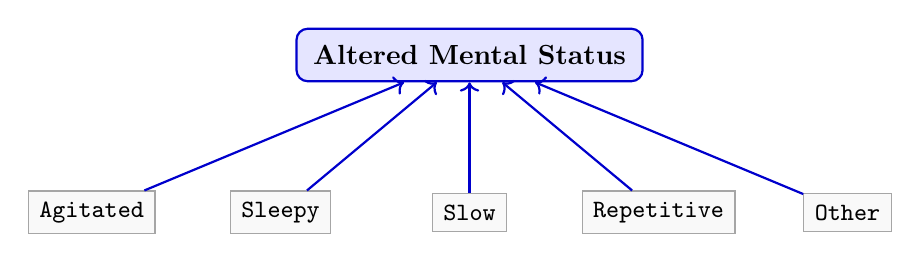
\begin{tikzpicture}[
            grow=down,
            level 1/.style={level distance=2.0cm, sibling distance=2.4cm},
            edge from parent/.style={draw=blue!80!black, <-, thick},
            root/.style={rectangle, rounded corners, draw=blue!80!black, fill=blue!10, thick, font=\bfseries, inner sep=6pt},
            leaf/.style={rectangle, draw=gray!70, fill=gray!5, font=\ttfamily\small, inner sep=4pt}
        ]
            \node[root] {Altered Mental Status}
                child { node[leaf] {Agitated} }
                child { node[leaf] {Sleepy} }
                child { node[leaf] {Slow} }
                child { node[leaf] {Repetitive} }
                child { node[leaf] {Other} };
        \end{tikzpicture}%
    }
    \caption{Altered Mental Status Hierarchy}
    \label{fig:ams_hierarchy}
\end{figure}



For example, altered mental status is represented by a primary indicator together with several more specific manifestations (Figure 2). When a component indicates an altered mental state, the corresponding overall indicator can be inferred without introducing a statistical model or an assumption about the prevalence of the condition. Similar relationships occur throughout the data, including the relationship between the total Glasgow Coma Score (GCS) and its eye, verbal, and motor components. \\

These relationships are useful not only for imputation but also for checking the internal consistency of the recorded data. When multiple variables describe the same clinical feature, disagreement between them provides evidence that an observation requires attention during cleaning. Conversely, agreement provides additional support for the recorded value. Thus, the hierarchical structure of the clinical variables provides information about the data-generating process that would be lost if each variable were cleaned independently. Due to distinction between broad clinical indicator variables and their more specific component variables, we treat the indicator variables as the primary representation of a clinical finding. From a clinical data-collection perspective, these variables are generally the simplest observations to record: a clinician can indicate whether a finding is present or absent without necessarily documenting every specific manifestation or characteristic of that finding. The component variables provide additional clinical detail, but require a more granular assessment and may therefore be missing even when the broader clinical finding has been observed.\\

This distinction informs the hierarchy used during data cleaning. When the component variables provide sufficient information to determine a missing indicator, we use them to reconstruct the indicator. However, when there is a conflict between an indicator and its components, we do not automatically treat the more detailed component variables as the more reliable observation. Instead, the indicator is given priority because it represents the primary clinical assessment and is more closely aligned with how the finding would be recorded in practice.\\

This approach is particularly relevant for the PECARN data because the ultimate purpose of the variables is to support a clinical decision rule. The question faced by a clinician is often fundamentally binary: does this child exhibit the clinical feature or not? The additional component variables help describe \textit{how} the feature manifests, but the indicator captures the clinical determination that is most directly relevant to the decision-making process.




\subsubsection{Dealing with Ambiguity Arising from Missing information}

While some variables have a clean (or cleaner) structure as discussed in the previous section, there are some variables without a clear linear hierarchical. One such example is in the mechanism of injury variable which has a direct correspondence to the severity of mechanism of injury vairable. Kupperman et al. explain how the severity of the mechanism is derived from the mechanism itself though a collection of rules 
\ref{fig:injury_severity_rules}. 


\begin{figure}[htbp]
\centering
\resizebox{0.6\linewidth}{!}{%
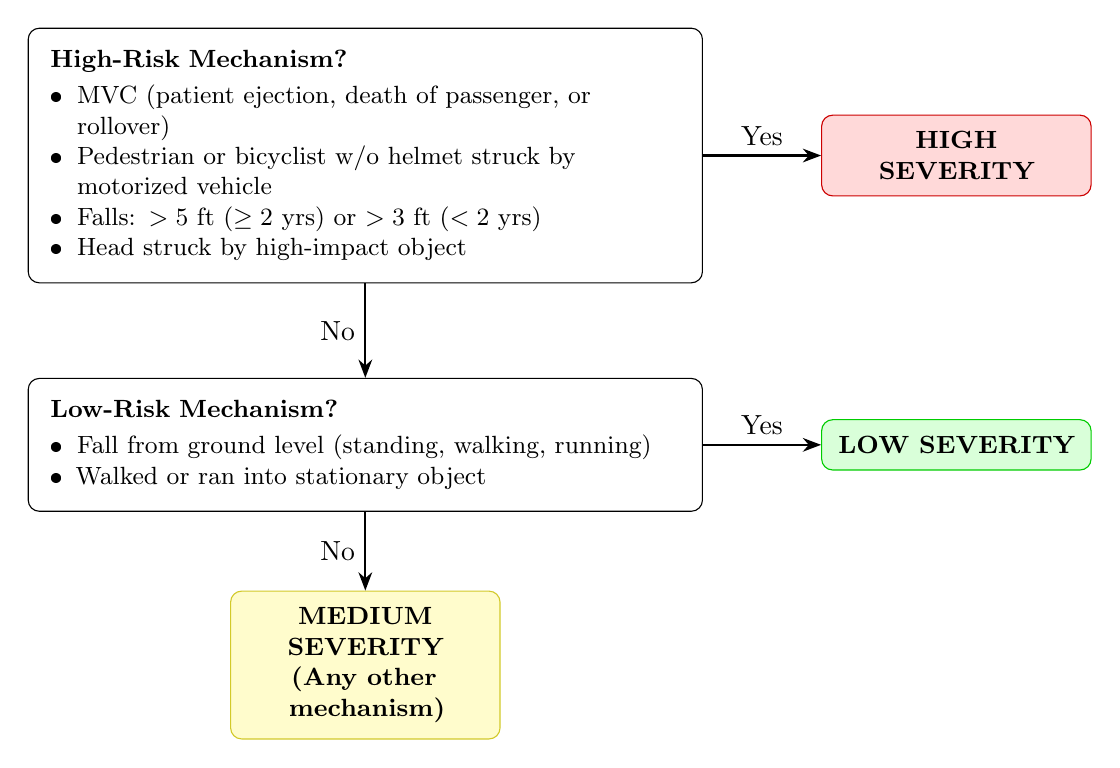
\begin{tikzpicture}[
    node distance=1.8cm,
    block/.style={rectangle, draw, rounded corners, text width=8cm, align=left, inner sep=8pt, font=\small},
    decision/.style={diamond, draw, text width=4.5cm, align=center, inner sep=4pt, font=\small},
    outcome/.style={rectangle, draw, rounded corners, text width=3cm, align=center, font=\bfseries\small, inner sep=6pt},
    arrow/.style={-Stealth, thick}
]

% Nodes
\node (decision1) [block] {\textbf{High-Risk Mechanism?}
\begin{itemize}[leftmargin=*,noitemsep,topsep=2pt]
    \item MVC (patient ejection, death of passenger, or rollover)
    \item Pedestrian or bicyclist w/o helmet struck by motorized vehicle
    \item Falls: $>5$ ft ($\ge 2$ yrs) or $>3$ ft ($< 2$ yrs)
    \item Head struck by high-impact object
\end{itemize}};

\node (high) [outcome, fill=red!15, draw=red!80!black, right=1.5cm of decision1] {HIGH SEVERITY};

\node (decision2) [block, below=1.2cm of decision1] {\textbf{Low-Risk Mechanism?}
\begin{itemize}[leftmargin=*,noitemsep,topsep=2pt]
    \item Fall from ground level (standing, walking, running)
    \item Walked or ran into stationary object
\end{itemize}};

\node (low) [outcome, fill=green!15, draw=green!80!black, right=1.5cm of decision2] {LOW SEVERITY};
\node (med) [outcome, fill=yellow!20, draw=yellow!80!black, below=1cm of decision2] {MEDIUM SEVERITY\\(Any other mechanism)};

% Paths
\draw [arrow] (decision1) -- node[anchor=south] {Yes} (high);
\draw [arrow] (decision1) -- node[anchor=east] {No} (decision2);
\draw [arrow] (decision2) -- node[anchor=south] {Yes} (low);
\draw [arrow] (decision2) -- node[anchor=east] {No} (med);

\end{tikzpicture} }
\caption{Decision rule tree for injury severity classification based on mechanism.}
\label{fig:injury_severity_rules}
\end{figure}

We do not have information for many of these decision rules. We do not have any data if there were fatalities in the motor vehicle crash (MVC); nor do we know the height of the fall.
This leads to the discrepancies we can observe in Figure \ref{fig:injury_mech} where we see multiple different severties are attributed to one type of injury.  

\begin{figure}[H]
    \centering
    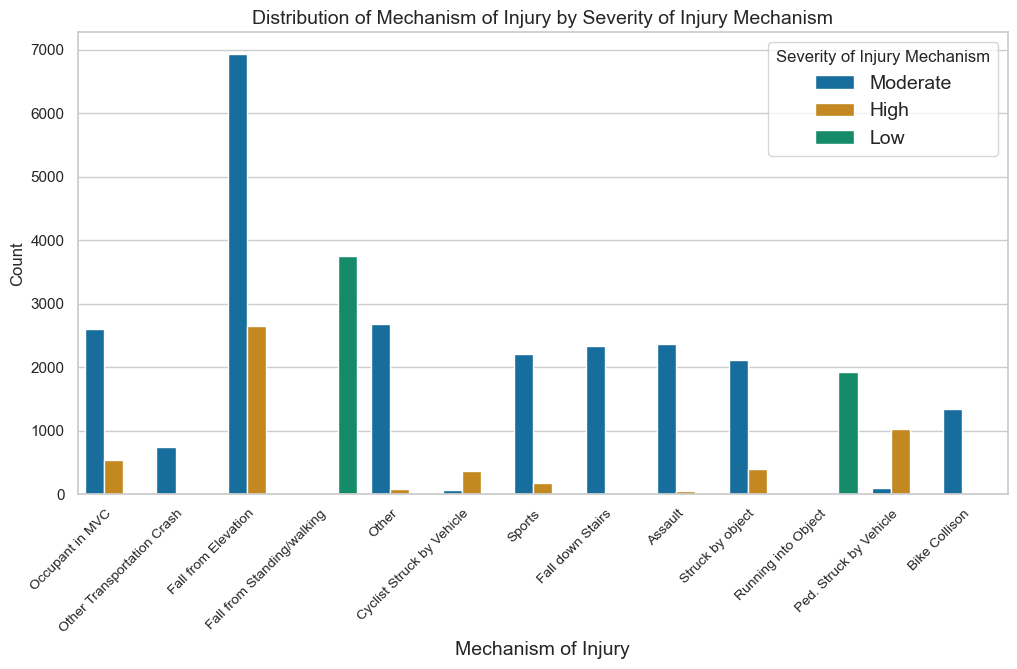
\includegraphics[width=.8\linewidth]{../figs/injury_mechanism.png}
    \caption{Injury mechanism severity grouped by the mechanism of injury; note that there are different injury mechanism severity within different mechanisms. This discrepancy is the product of outside information.}
    \label{fig:injury_mech}
\end{figure}

Therefore, in order to impute possible missing values in the severity of injury mechanism, we create a possible permutation in the cleaning process, allow for greater caution or less caution. Greater caution means that if it is unclear is a motor vehicle crash was severe (based on the rules described above) then the assumption is that it was severe.
Conversely, if there is an assumption that most motor vehicle crashes are not severe, then we can permute the cleaning to map such cases to a moderate severity.\\

We create a similar functionality in the cleaning to deal an assumption made by Kuppermann et al. that was attributed to small sample size and also included domain specific knowledge surrounding the Glasgow Coma Score. 
Kuppermann et al. remove those patients with a GCS of less than fourteen from the analysis. This assumption places an inherent reliance on the effectivity of the Glasgow Come Score across age groups despite the test varying between
preverbal and verbal children (which in the context of this problem is translated to older than or younger than two years old). For this reason we create a possible perturbation in the whether or not to include patients with a 
Glasgow score under 14. The impacts of this decision are considered in Section \ref{stability-check}.

\renewcommand{\arraystretch}{1.2}
\setlength{\tabcolsep}{5pt}
\small

\begin{xltabular}{\linewidth}{
    >{\bfseries\color{navyheader}}p{2.5cm}
    p{3.2cm}
    >{\ttfamily\color{paramcolor}}p{3.2cm}
    X
}\label{tab:data-cleaning-summary} 

\caption{Summary of Clinical Cleaning Rules and Pipeline Input Parameters}
\\

\toprule
\rowcolor{navyheader}
\textcolor{white}{Domain} &
\textcolor{white}{Variables} &
\textcolor{white}{Pipeline Parameter} &
\textcolor{white}{Cleaning Rules \& Imputation Logic} \\
\midrule
\endfirsthead

% Repeat only the column header on subsequent pages
\toprule
\rowcolor{navyheader}
\textcolor{white}{Domain} &
\textcolor{white}{Variables} &
\textcolor{white}{Pipeline Parameter} &
\textcolor{white}{Cleaning Rules \& Imputation Logic} \\
\midrule
\endhead

% No footer on page breaks
\endfoot

% Bottom of the final page
\bottomrule
\endlastfoot

Age &
\texttt{agetwoplus}, \texttt{ageinmonth} &
\normalfont--- &
\textbf{Threshold Imputation:} Imputes missing indicator using age in months
($<24$ mo $\rightarrow$ 'Younger than 2', $\ge 24$ mo $\rightarrow$ '2 or Older'). \\
\rowcolor{rowaccent}

GCS Scores &
\texttt{gcstotal}, \texttt{gcseye}, \texttt{gcsverbal},
\texttt{gcsmotor}, \texttt{gcsgroup} &
include\_severe\_cases \newline\small(Default: False) &
\begin{itemize}[label={}, leftmargin=0pt, labelwidth=0pt, itemindent=0pt, nosep]
  \item[]\textbf{Summation:} Recalculates total GCS from subscores; aligns severity group
  ($<14 \rightarrow$ Severe, $\ge 14 \rightarrow$ Moderate).
  \item[] \textbf{Max Imputation:} If total GCS == 15 but subscores missing,
  sets max values (eye=4, verbal=5, motor=6).
  \item[] \textbf{Parameter Switch:} Toggles whether severe cases ($<14$)
  are retained or dropped from the cohort.
\end{itemize} \\

Altered Mental State &
\texttt{ams}, \texttt{amsagitated}, \texttt{amssleep},
\texttt{amsslow}, \texttt{amsrepeat}, \texttt{amsoth} &
\normalfont--- &
\textbf{Symptom Inferencing:} Imputes 'Yes' if any subvariable is positive
or total GCS $<15$. Imputes 'No' if subvariables are missing and GCS == 15. \\
\rowcolor{rowaccent}

Hematoma &
\texttt{hema}, \texttt{hemaloc}, \texttt{hemasize} &
\normalfont--- &
\textbf{Back-Imputation:} Imputes overall flag as 'Yes' if location or size
is specified; imputes 'No' if both are missing. \\

Loss of Consciousness &
\texttt{locseparate}, \texttt{loclen} &
suspected\_loc \newline\small(Default: False) &
\textbf{Parameter Switch:} If \texttt{False}, nullifies duration for
'Suspected' cases. If \texttt{True}, retains reported duration intervals.
Back-imputes overall flag as 'Yes' if duration is present. \\
\rowcolor{rowaccent}

Mechanism of Injury &
\texttt{injurymech}, \texttt{high\_impact\_injsev} &
extreme\_caution \newline\small(Default: False) &
\textbf{Parameter Switch:} Controls fallback severity for missing values.
Imputes 'High' if \texttt{True}; defaults to 'Moderate' if \texttt{False}
(high-impact auto-maps to 'High', low-impact to 'Low'). \\

Skull Fracture &
\texttt{sfxpalp}, \texttt{sfxpalpdepress}, \texttt{sfxbas} &
\normalfont--- &
\textbf{Logical Consistency:} Imputes overall fracture to 'Yes' if any
sub-variable is positive. Sets missing palpable to 'Unclear' and missing
basilar to 'No'. \\
\rowcolor{rowaccent}

Fontanelle Bulging &
\texttt{fontbulg} &
\normalfont--- &
\textbf{Epidemiological Imputation:} Imputes missing values as 'No'
based on clinical rarity. \\

Headache &
\texttt{ha\_verb}, \texttt{haseverity}, \texttt{hastart} &
\normalfont--- &
\textbf{Attribute Inferencing:} Imputes verbal status as 'Yes' if headache
severity is populated. \\
\rowcolor{rowaccent}

Vomiting &
\texttt{vomit}, \texttt{vomitnbr}, \texttt{vomitstart}, \texttt{vomitlast} &
\normalfont--- &
\textbf{Cross-Field Inferencing:} Sets overall flag to 'Yes' if episode
counts or timing fields are populated; otherwise imputes 'No'. \\

Dizzy \& Acting Normal &
\texttt{dizzy}, \texttt{actnorm} &
\normalfont--- &
\textbf{Preservation:} Preserves missing values without making clinical assumptions. \\
\rowcolor{rowaccent}

Outcome (ciTBI) &
\texttt{posintfinal} &
\normalfont--- &
\textbf{Complete Case Filter:} Filters out records with missing primary
outcome values prior to cohort generation. \\

\end{xltabular}


\subsubsection{Notes of Limitations of Cleaning Procedure}

As previously noted, the missing information in this data created inherent limitations on imputing missing values. With that is the issue of imputing missing outcome values: whether or not a patient was diagnosed with a ciTBI.
Since we are unable to fill in this information with any provided information, and due to the poignance of the reliability of the outcome, we elect to remove patients with missing outcome from the analysis.\\

Additionally, due to time and cognitive budget constraints, only those variables and subvariables considered in Kuppermann et al. were cleaned. We feel this is an acceptable condition in light of the domain expertise presented by Kuppeermann et al.
as clinicians, the variables they consider are those that we can only assume to be of both clinical significance, and reasonably obtainable by an emergency care giver in a stressful, high impact environment. 
We seek to  maintain the applicability of this analysis to practice. In future work, there may be deeper considerations that would, under domain informed advice, prove valuable.

\subsection{Data Exploration}\label{data-exploration}

To gain a better understanding of the data and the structures suggested by Kuppermann et al. we complete a more extensive data exploration. As the Glasgow Coma Score is an important factor for determining inclusion in the study. With that comes the natural issue in the differences between the way that GCS are derived from children of different ages. We explore the data to see if the way that GCS is addressed in the study is appropriate. In Figure \ref{fig:gcs_by_age} we look at the distribution of GCS by age.


\begin{figure}[H]
    \centering
    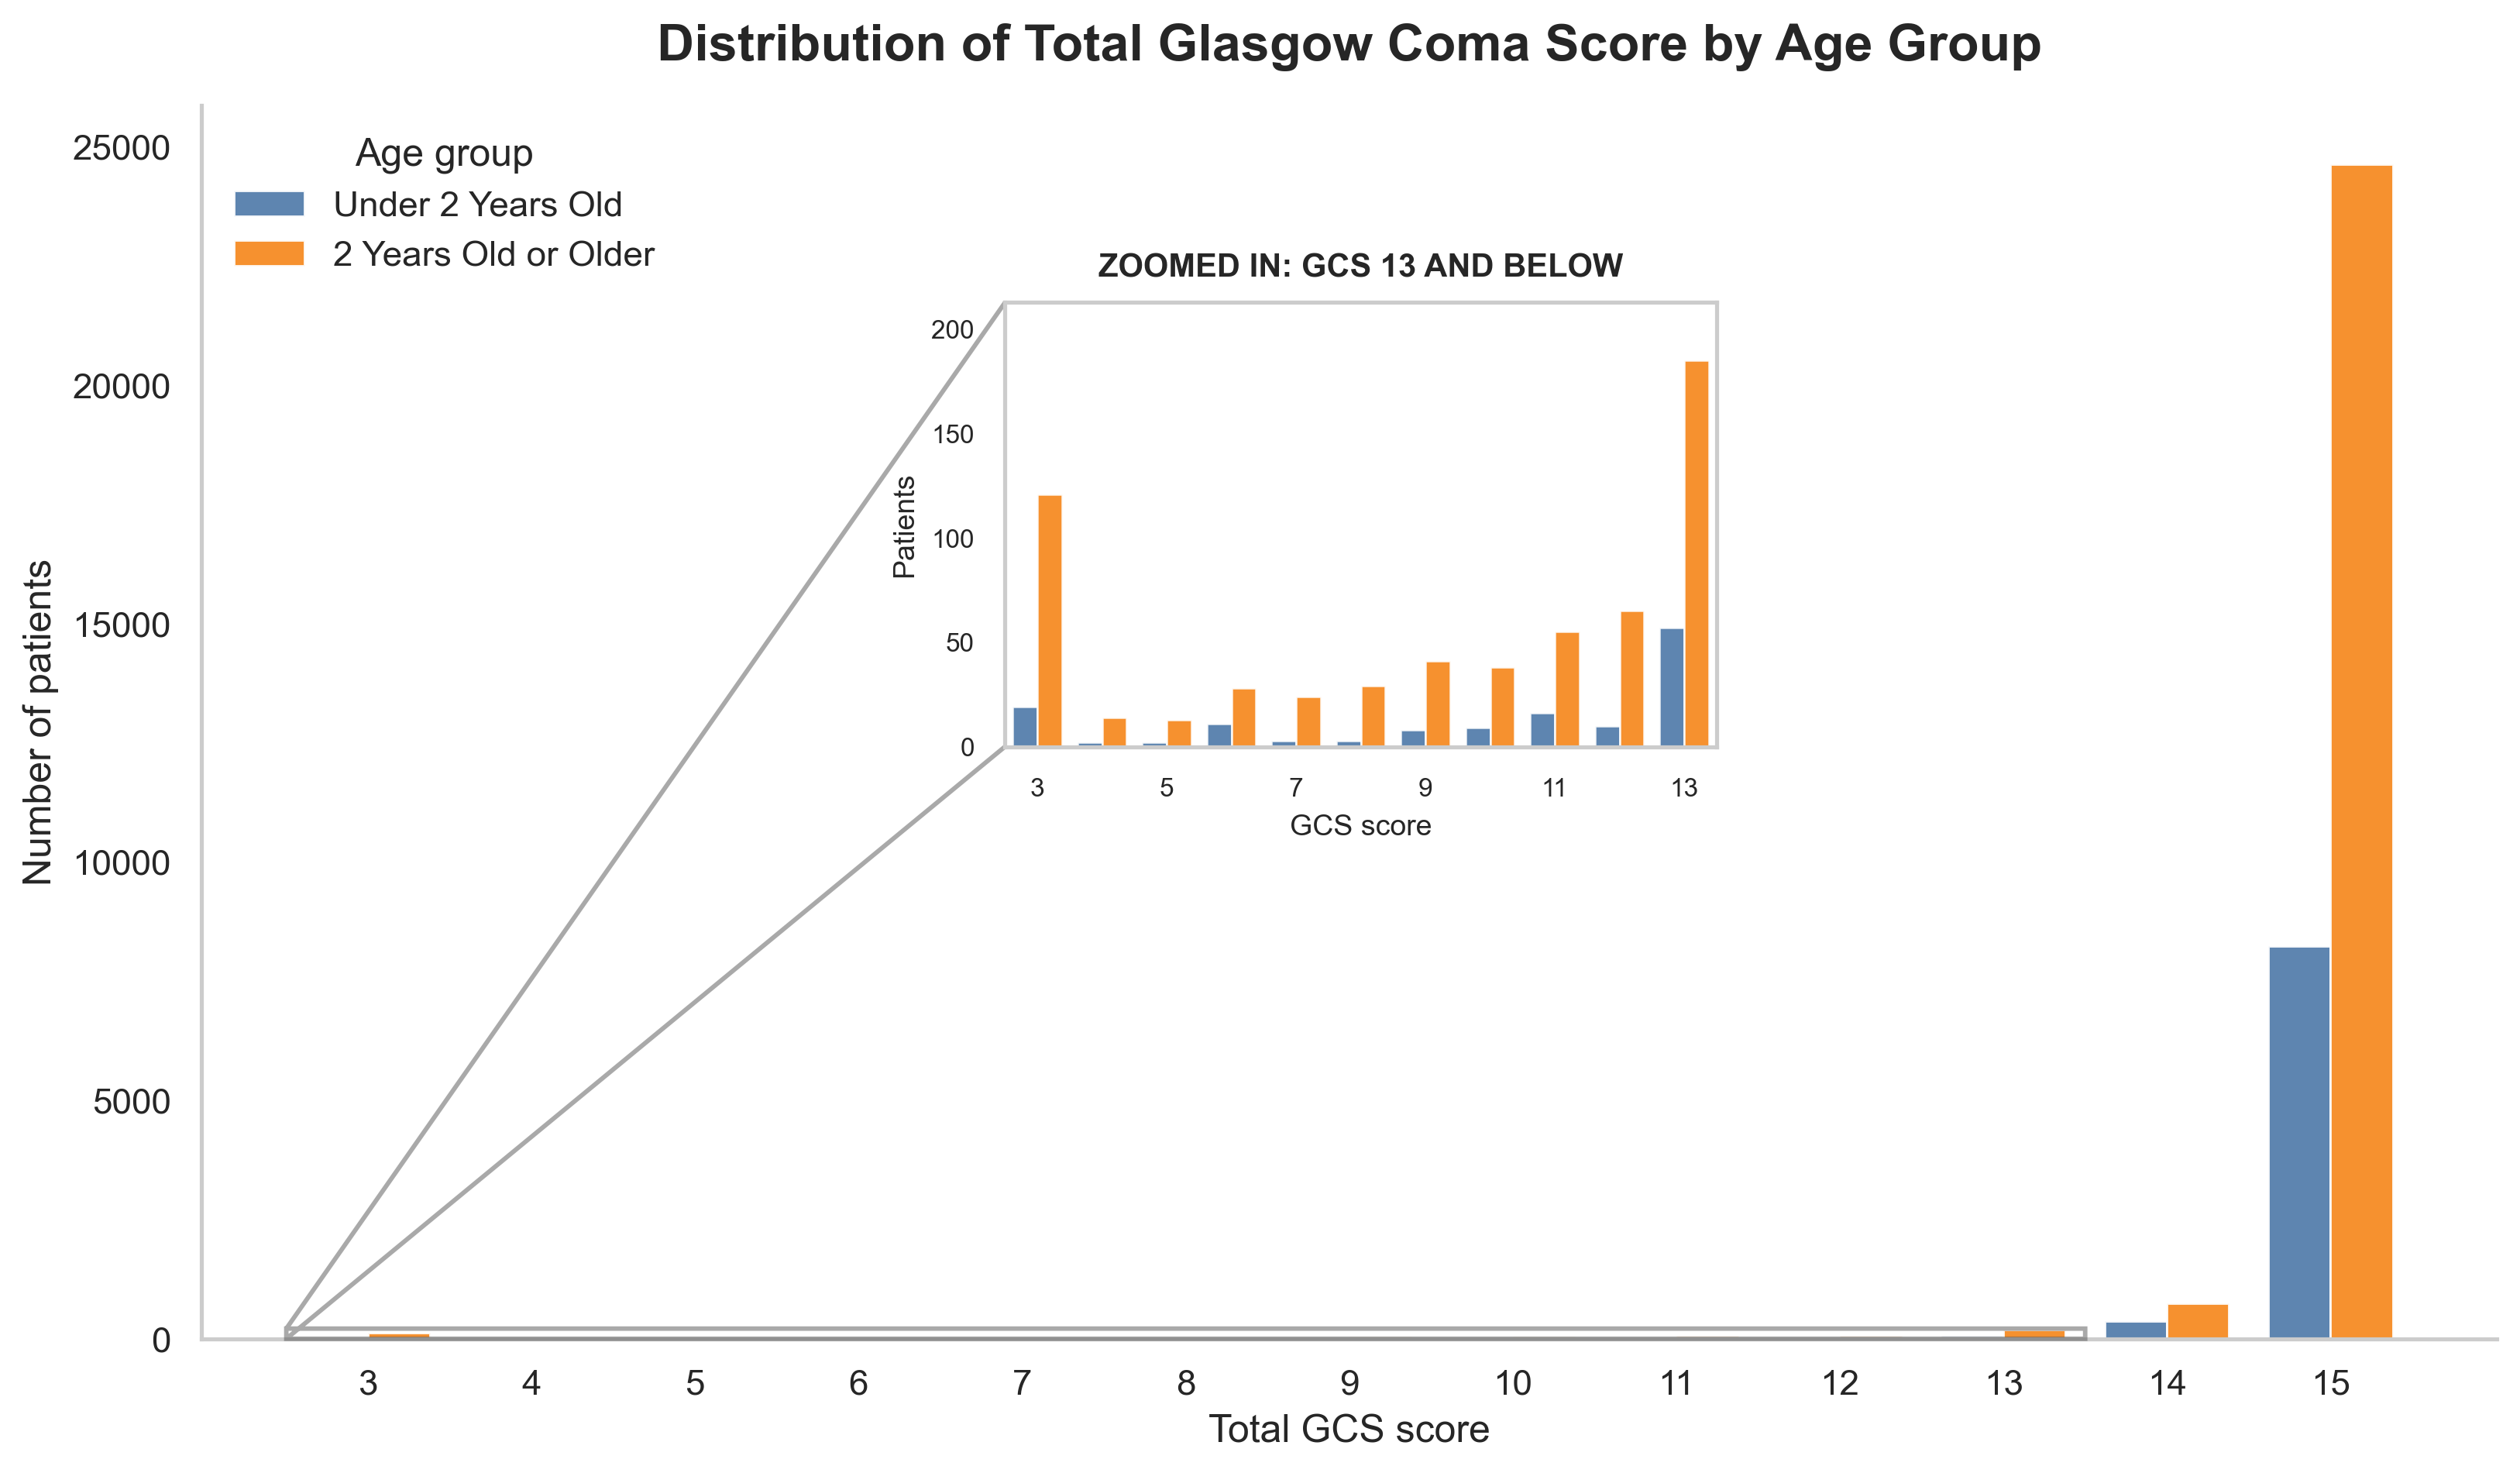
\includegraphics[width=0.75\linewidth]{../figs/gcs_total_distribution_by_age.png}
    \caption{Caption}
    \label{fig:gcs_by_age}
\end{figure}

We must be very careful about what conclusions we can draw from this figure as there are substantially more children older than two years old in the study. However it is interesting to observe the distribution in GCS values as there is a clear, and not unexpected downward trend corresponding to a decrease in GCS (which represents an increase in symptom severity). \\

At the very heart of this issue is the difference in behavior and cognitive ability of a child. This has a massive impact on the quality and structure of the assessment of a head injury. We visualize how altered mental status indicators are distributed differently by age in Figure \ref{fig:ams_by_age}.

\begin{figure}[H]
    \centering
    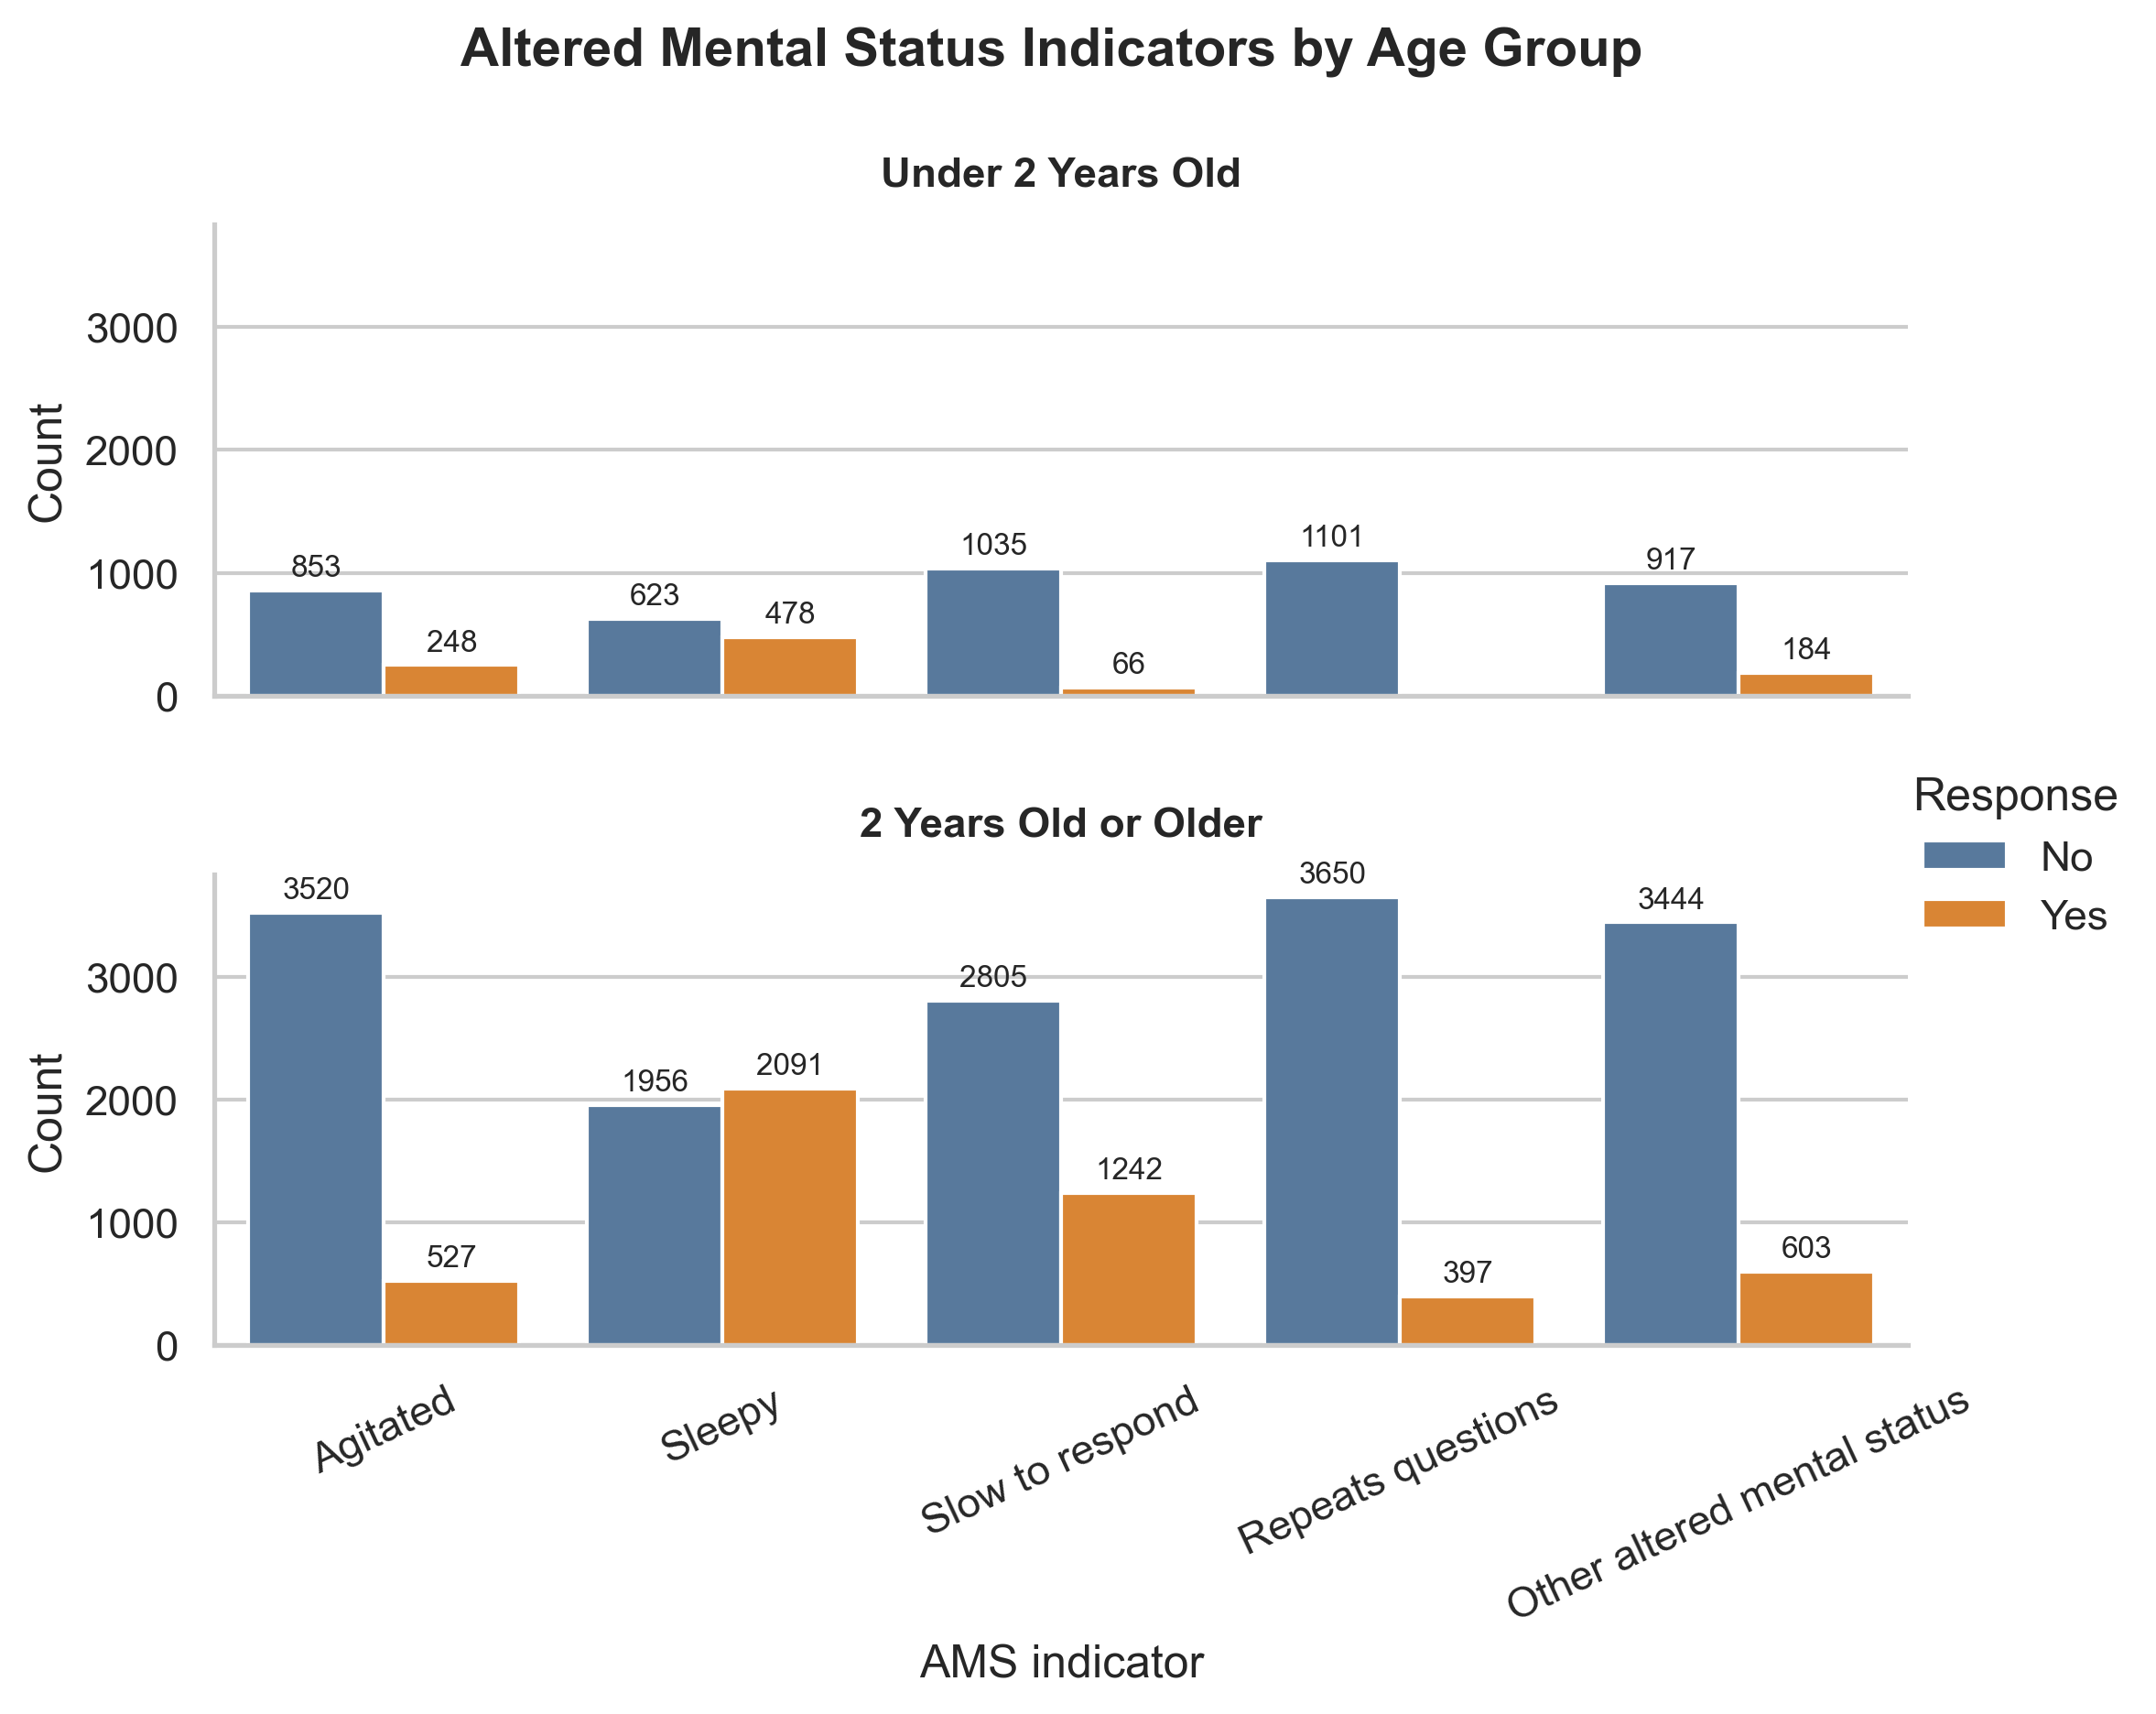
\includegraphics[width=.7\linewidth]{../figs/AMS_indicators_by_age_group.png}
    \caption{Altered mental status indicators by age}
    \label{fig:ams_by_age}
\end{figure}

Again, not unexpectedly, children under two cannot be evaluated on how the respond to questions if they are preverbal. As such that will not show up in an examination. Other than these obvious shortcomings, the distributions seem to follow similar behavior which points to the robustness of the clinical evaluations, despite the extreme gap in developmental stage. 

\section{Findings}\label{findings}

The observations presented in the exploratory data analysis indicate that the decision rule based on age might not carry as much weight as indicated by Kuppermann et al. Whether that implies that a more granular separation of age is necessary or not is worth considering when dealing with GCS. Moreover, it is worth examining how the proportion of ciTBI change based on age. Both of these questions are addressed in this section.

\subsection{First finding}\label{first-finding}
We first consider how granularity of age might impact the reliability of GCS. In Figure \ref{fig:mean_gcs_byage} we present two versions of the same plot. The top plot shows the arithmetic mean GCS by age in years with all GCS less than thirteen removed from the data set as per the specifications of Kuppermann et al. While we cannot assess the variability of children under two years old in this plot (as there are only two points), we see that there does not appear to be evidence to indicate that there is a particularly different manifestation of the GCS between young children and older children.

We compare this to the bottom plot which gives the same information however we have increased the granularity by showing the average GCS by age in months. What appears is an interesting heteroskedastic trend: variability increases with age. This is certainly not due to change in how the GCS is ascertained since the variability primarily changes in older children. This is likely because of the greater variety of incidents that older children may be exposed to which result in head injury. Events such as car accidents, sports injuries, or even events involved with drugs or intoxication become more prevalent in the older children. Unfortunately, this is a case where have the time time series data would be valuable. It would be interesting to see if there is any seasonal structure within these age groups. For example, perhaps here are more severe head injuries in football season for older children or more severe injuries in the winter from slipping on ice. 

\begin{figure}[H]
    \centering
    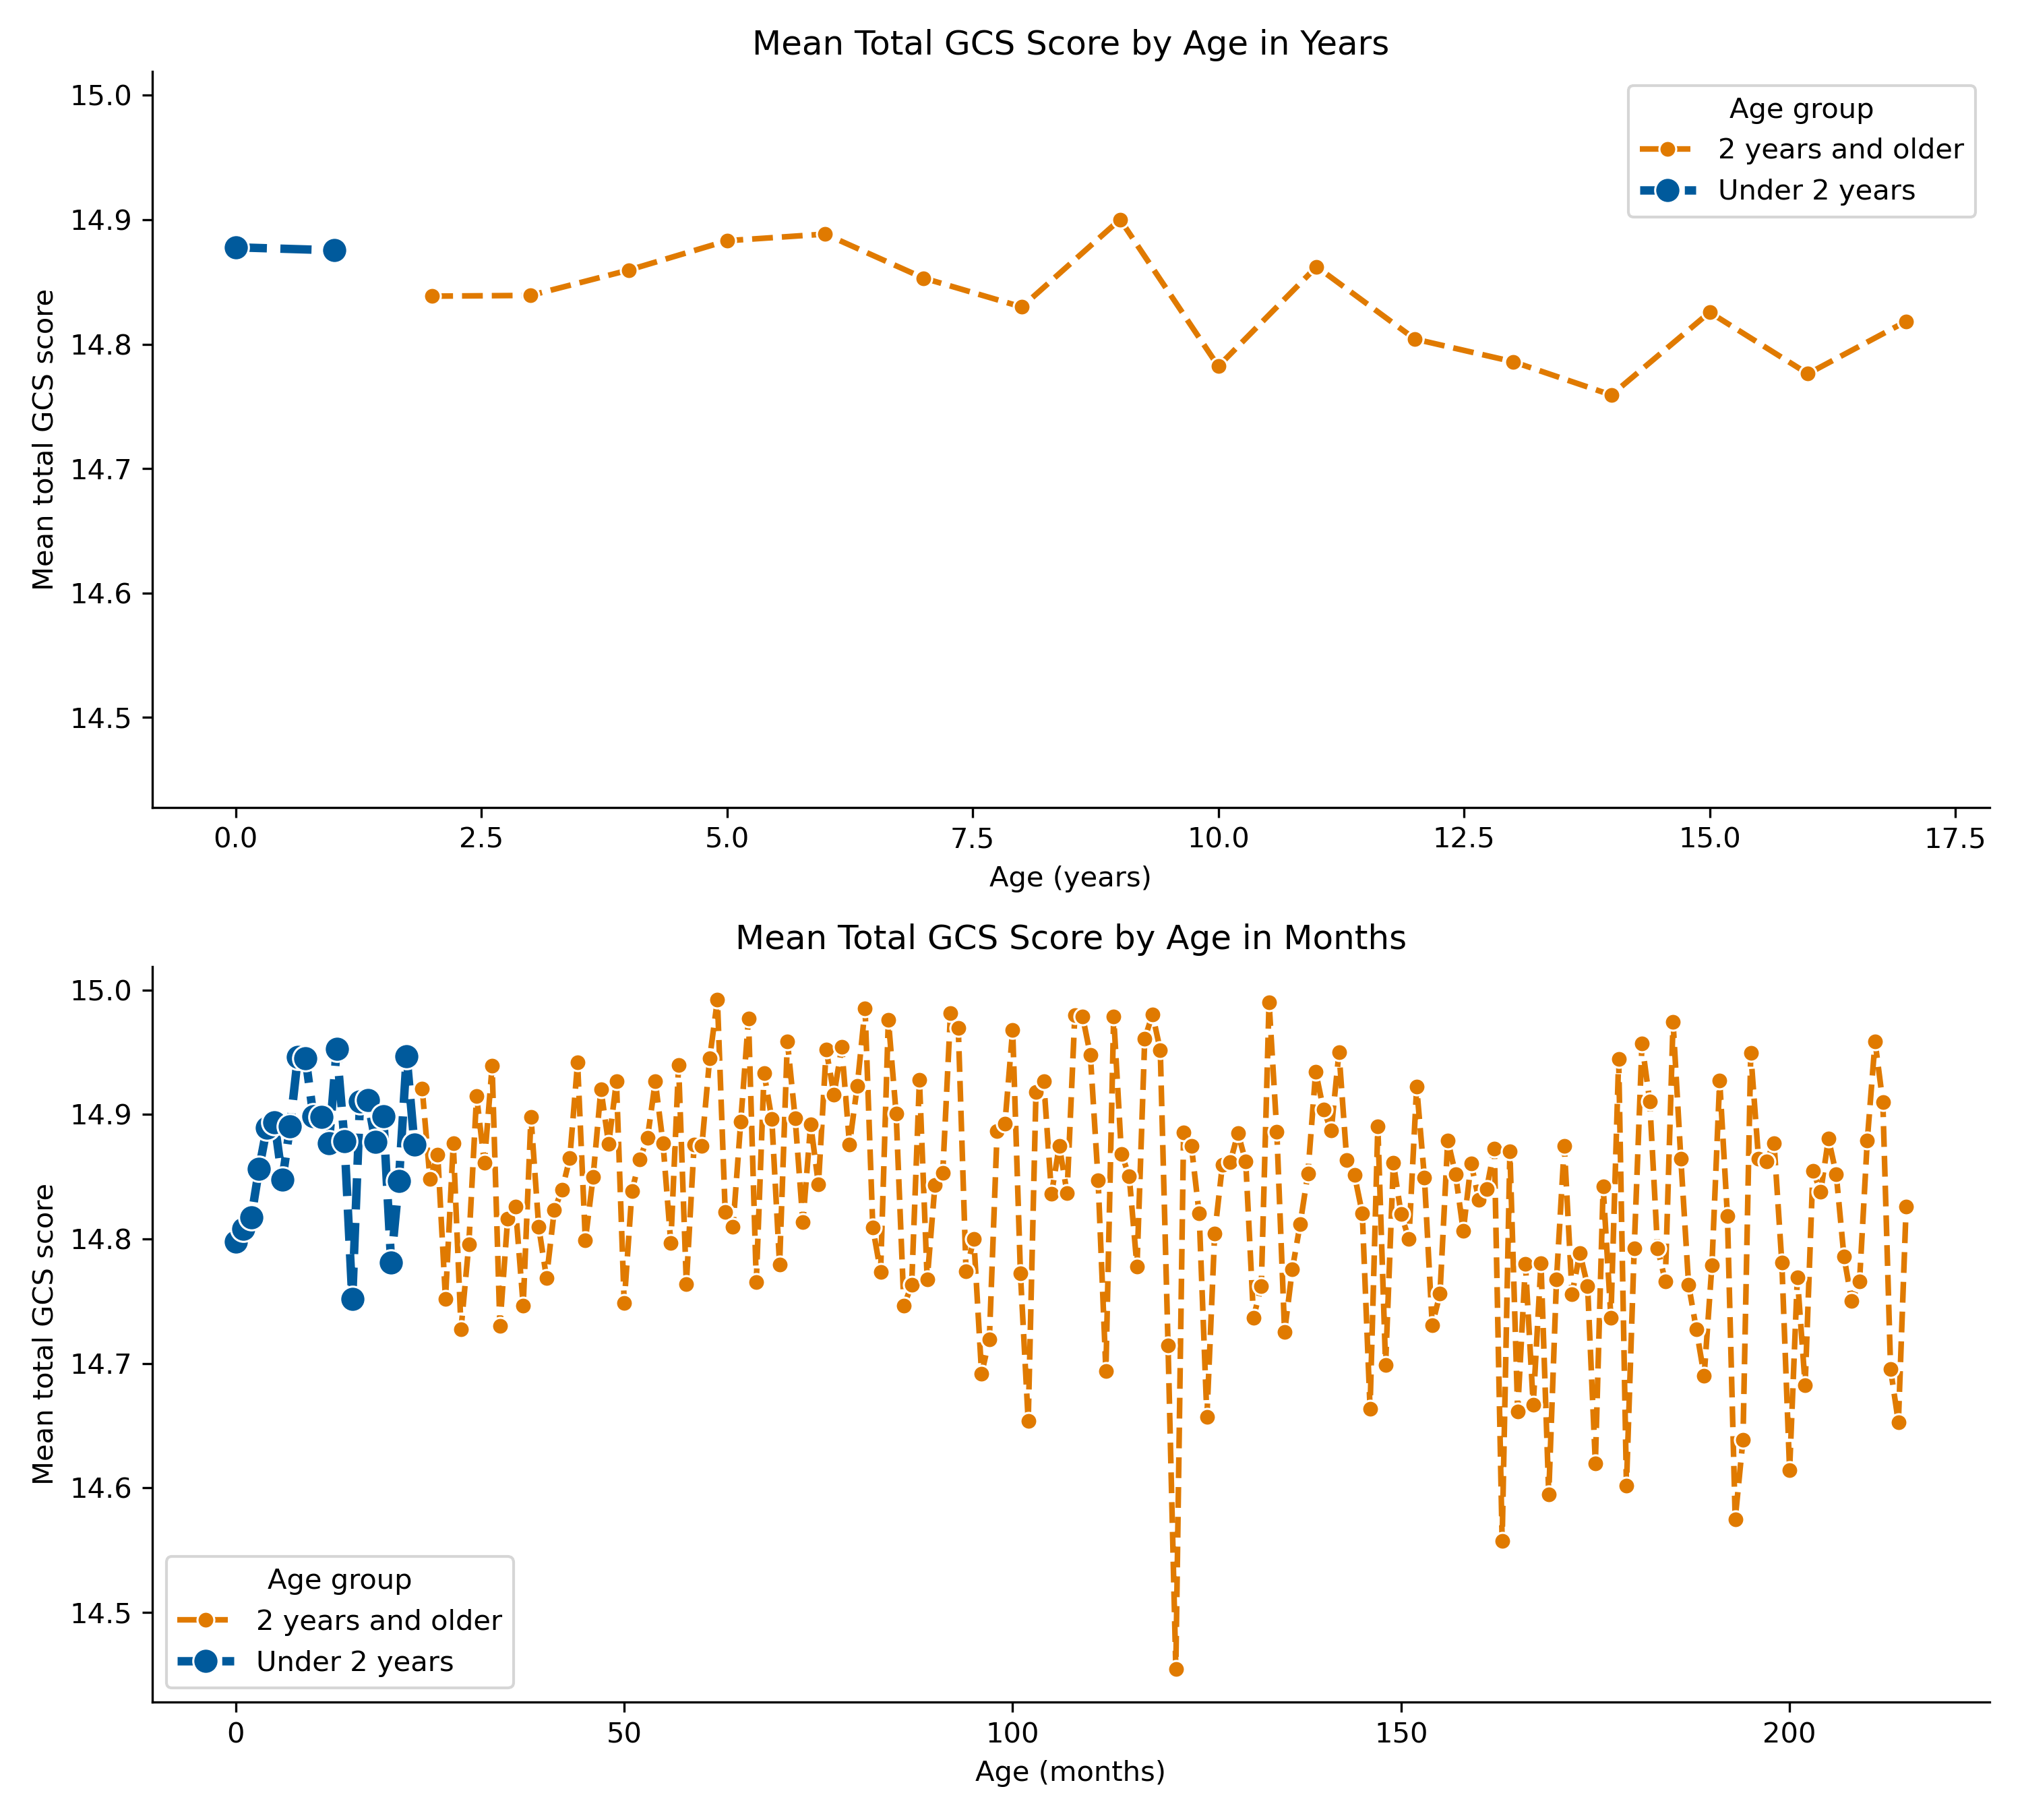
\includegraphics[width=0.7\linewidth]{../figs/mean_gcs_by_age.png}
    \caption{Mean GCS by Age in Years (Top) and Age in Months (bottom)}
    \label{fig:mean_gcs_byage}
\end{figure}

\subsection{Second finding}\label{second-finding}

We next consider how the proportion of ciTBI changes based on between children youn ger than two and children aged two and over in Figure \ref{fig:ciTBI_propo_default}. We still use data under the assumptions of Kuppermann et al. where we have removed those with a GCS score of less than thirteen. Figure \ref{fig:ciTBI_propo_default} highlights two important features. The first is that ciTBI is 

\begin{figure}[H]
    \centering
    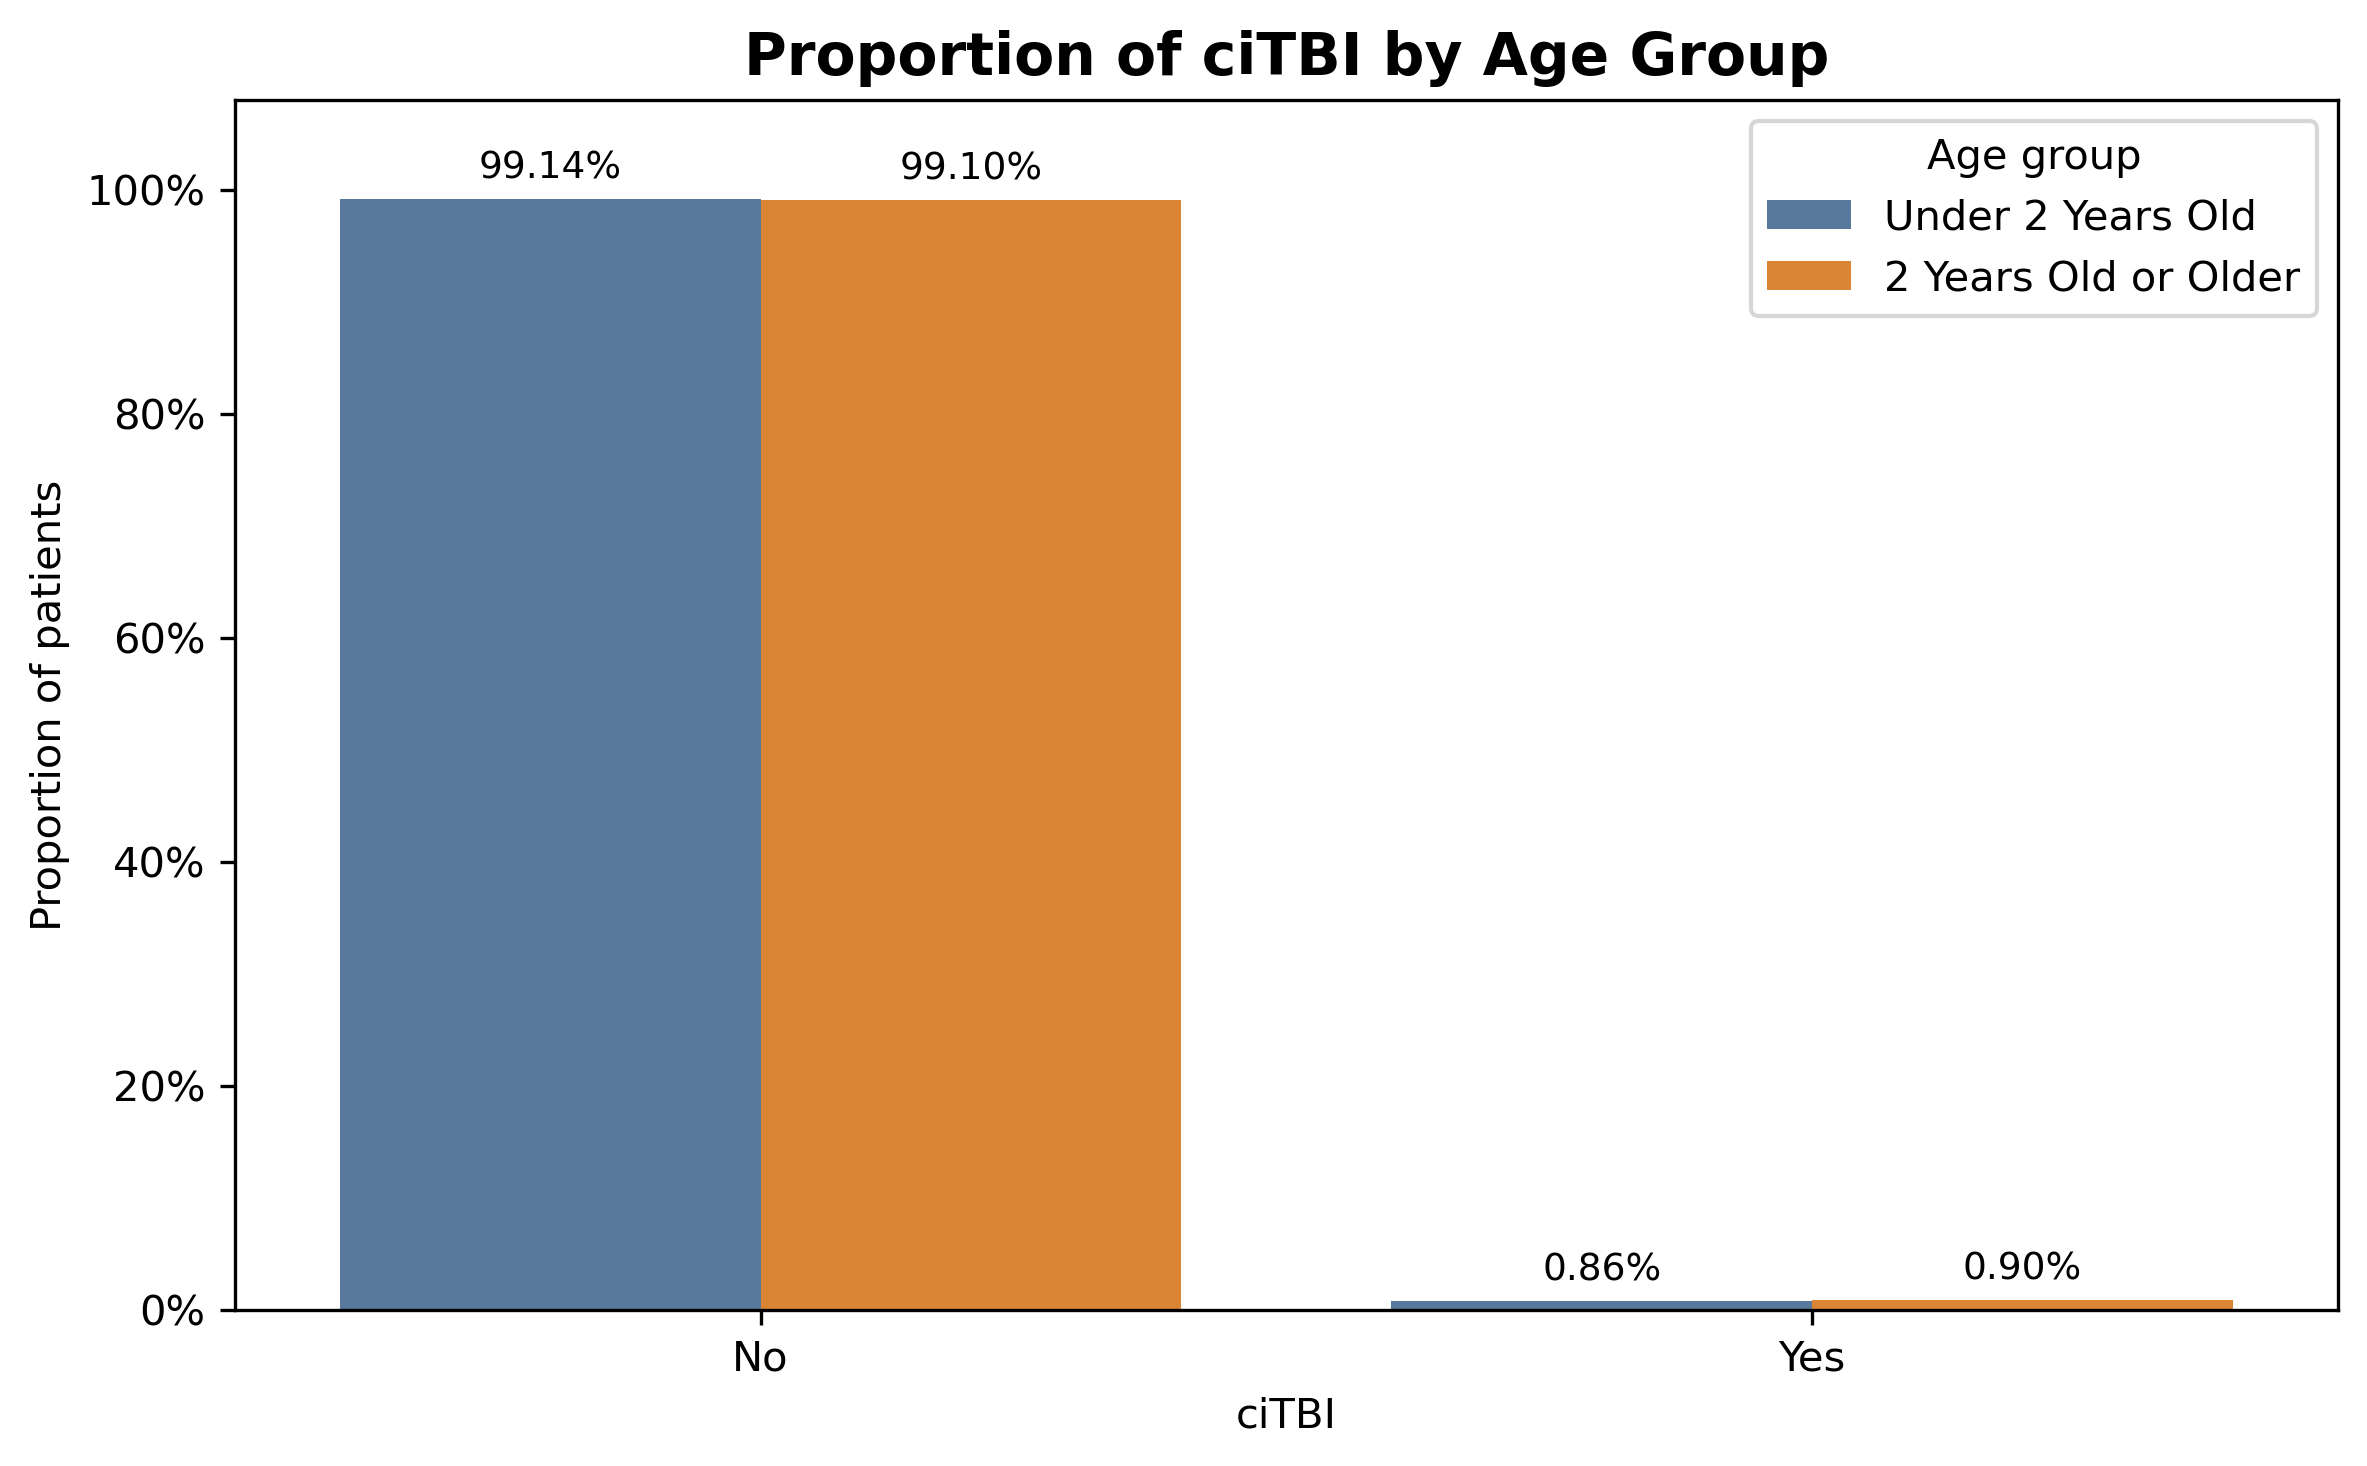
\includegraphics[width=0.6\linewidth]{../figs/ciTBI_proportion_by_age_group_GCS_excluded.png}
    \caption{}
    \label{fig:ciTBI_propo_default}
\end{figure}
 a rare event, making up only about one percent of all patients. This is important information which will be used in the modeling process (Section \ref{model}).\\

 Moreover, we can see that the proportions of ciTBI are extremely closely--within around a tenth of a percent of each other. This indicates that the way in which we evaluate younger children need not necessarily differ greatly from their older counterparts, as this information might be captured in the other variables. It is important to realize the by group children based on age is an attempt to classify children based on developmental stage, however not all children develop at the same rate. Perhaps by imposing such a strict boundary we are limiting the ability of the model to capture information that is more indicative of the true underlying biology and neurophysiology.  


\subsection{Reality Check}\label{reality-check}

The first part of the reality check is that none of these finding are particularly surprising given the domain context. We are considering the stability of the analysis across age where we find that there seems to be far more stability than expected. We find that certain variables which are collected for older children cannot be collected in younger children which is not surprising. Young children do not have the same verbal dn reasoning capacity to help medical professionals with their diagnosis. With that being said, that Kupperman et al. use this hard cutoff makes clinical sense. It is much more difficult to assess the developmental stage of a child, than to look at a birth date, or even to make a quick judgment call based on the the child being really young or not, at which point the cutoff at two becomes somewhat arbitrary. Thus, the nuance we uncover in these findings is not surprising.
  
\subsection{Stability Check}\label{stability-check}

Having made the decision to exclude patients with a GCS of less than thirteen, we present a stability check as both an evaluation of the choices made in data cleaning for this project but also a check on the assumptions presented by Kuppermann et al. We perturb the data cleaning to allow those patients with GCS of thirteen and below to be considered in the analysis and reproduce Figure \ref{fig:ciTBI_propo_default} to determine how much the ciTBI rate actaully chnages and thereby access the stability of exclduing this outlier, though minoirty, group from analysis. We consider cases with GCS of thirteen or lower to be ``Sever Cases" where as those between fourteen and fifteen are considered `Moderate".

\begin{figure}[H]
    \centering
    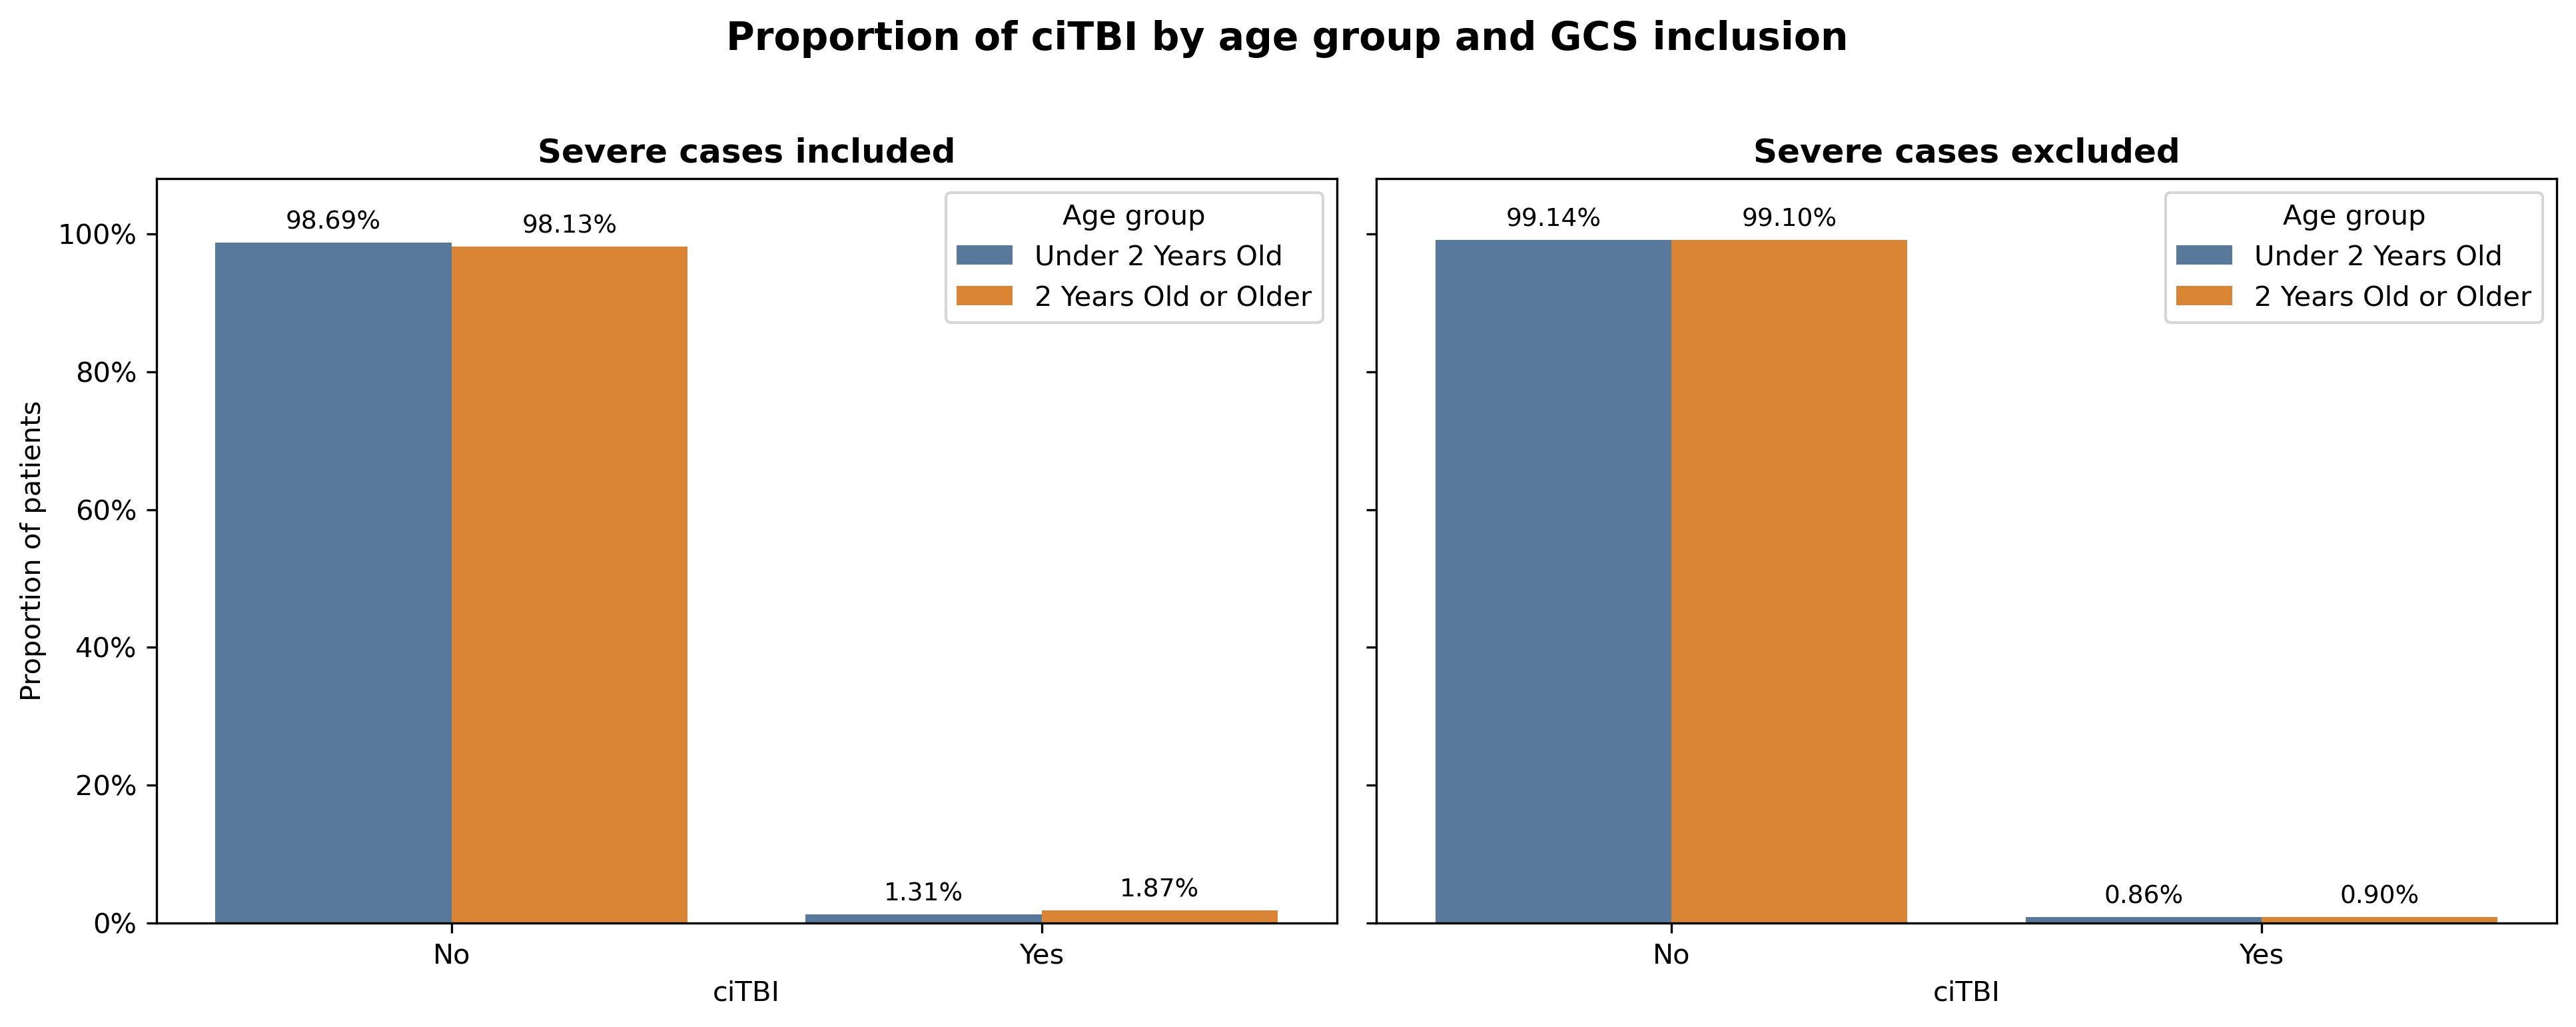
\includegraphics[width=.8\linewidth]{../figs/ciTBI_proportion_by_age_group_and_GCS_inclusion.png}
    \caption{Stability check of ciTBI rate by age}
    \label{fig:stability_check_finding}
\end{figure}

While at a first glance there does not seem to be very much difference, the change is rather large relativly speaking. By including the severe cases, we just about double the prevalence of our rare outcome in both age groups by only adding in $969$ observations. These are clearly high leverage data points with extreme significance. This is not necessarily unexpected behavior as those with low GCS are more severe cases and therefore are both more unlikely while presenting a higher rate of ciTBI diagnoses. That being said, the proportion of ciTBI cases is still very low. For this reason, the inclusion or exclusion of this subset needs to be taken into account when modeling in how we handle our rare outcome (Section \ref{model}). 

\section{Modeling}\label{model}

For the modeling procedure we considered tree based models in accordance with the ideas behind the decision rules presented by Kuppermann et al. The first model we ran was a simple Classification and Regression Tree. The second model is a Gradient Boosting Classifier. The CART provides excellent interpretability where as the Gradient Boosting approach conducts a wider search of the sample space. Both models and results are presented below. 

\subsection{Implementation}

We begin with the CART model which is the preferred presented in this paper due to its simplicity and interoperability. We tune the tree depth for our CART using 5-fold cross validation. Moreover, due to the rarity of the outcome variable we use balanced class weighting. Moreover, as we want to make sure that we identify those with ciTBI even if we have a higher false positive rate, we evaluate using Recall as a metric given by $$\text{Recall} = \frac{\text{True Positives}}{\text{True Positives} + \text{False Negatives}}$$ in both model selection and evaluation. Similarly, for the Gradient Boosting model, we train using 5-fold cross validation on all three hyperparameter: learning rate, maximum depth, and maximum iterations with ``Recall" as the decision metric.


\subsection{Stability and Results}
 In order to test the stability of the models as well as to assess the stability of the data cleaning choices made, we run the model on both data that includes patients with severe GCS (under thirteen) and with data that excludes those patients. Both models across both perturbations of the data sets had similarly underwhelming results (Table \ref{tab:model_performance}) compared to those presented by Kuppermann et al. \\

 \begin{table}[htbp]
  \centering
  \caption{Performance comparison of models across datasets.}
  \label{tab:model_performance}
  \begin{tabular}{l l c c}
    \toprule
    \textbf{Model} & \textbf{Dataset} & \textbf{Best CV Recall} & \textbf{Best Test Recall} \\
    \midrule
    \multirow{2}{*}{CART} 
      & Excluding Severe Cases & 0.732 & 0.824 \\
      & Including Severe Cases & 0.830 & 0.865 \\
    \midrule
    \multirow{2}{*}{Gradient Boosting} 
      & Excluding Severe Cases & 0.748 & 0.838 \\
      & Including Severe Cases & 0.820 & 0.871 \\
    \bottomrule
  \end{tabular}
\end{table}

What is most interesting about these findings is that the data set including severe cases seems to have produced a better predictor ciTBI in both the CART and Gradient Boosting models. While it is possible that there is a way in which the extreme GCS observations help train the model to recognize the symptoms of ciTBI as they are such clear examples. Conversely, consistent with the analysis in Section \ref{fig:stability_check_finding}, the improvement may be to a reduction in the rarity of the ciTBI outcome which improves model performance.\\

In addition to changes in the model performances there were also significant changes in the optimal model (as chosen through cross validation). The CART with severe cases excluded has depth of two, where as the corresponding tree for the data including severity is of depth three. The trade off between the complexity of the model and the accuracy of the classifications seems irrelevant in this case as both models are simple. For the Gradient Boosting model we also find a marginally more complex model for the data with severe cases included with learning rate of 0.2, maximum depth of 3, and maximum iterations of 50 compared to learning rate of 0.1, maximum depth of 3, and maximum iterations of 50.  

\begin{figure}[H]
    \centering
    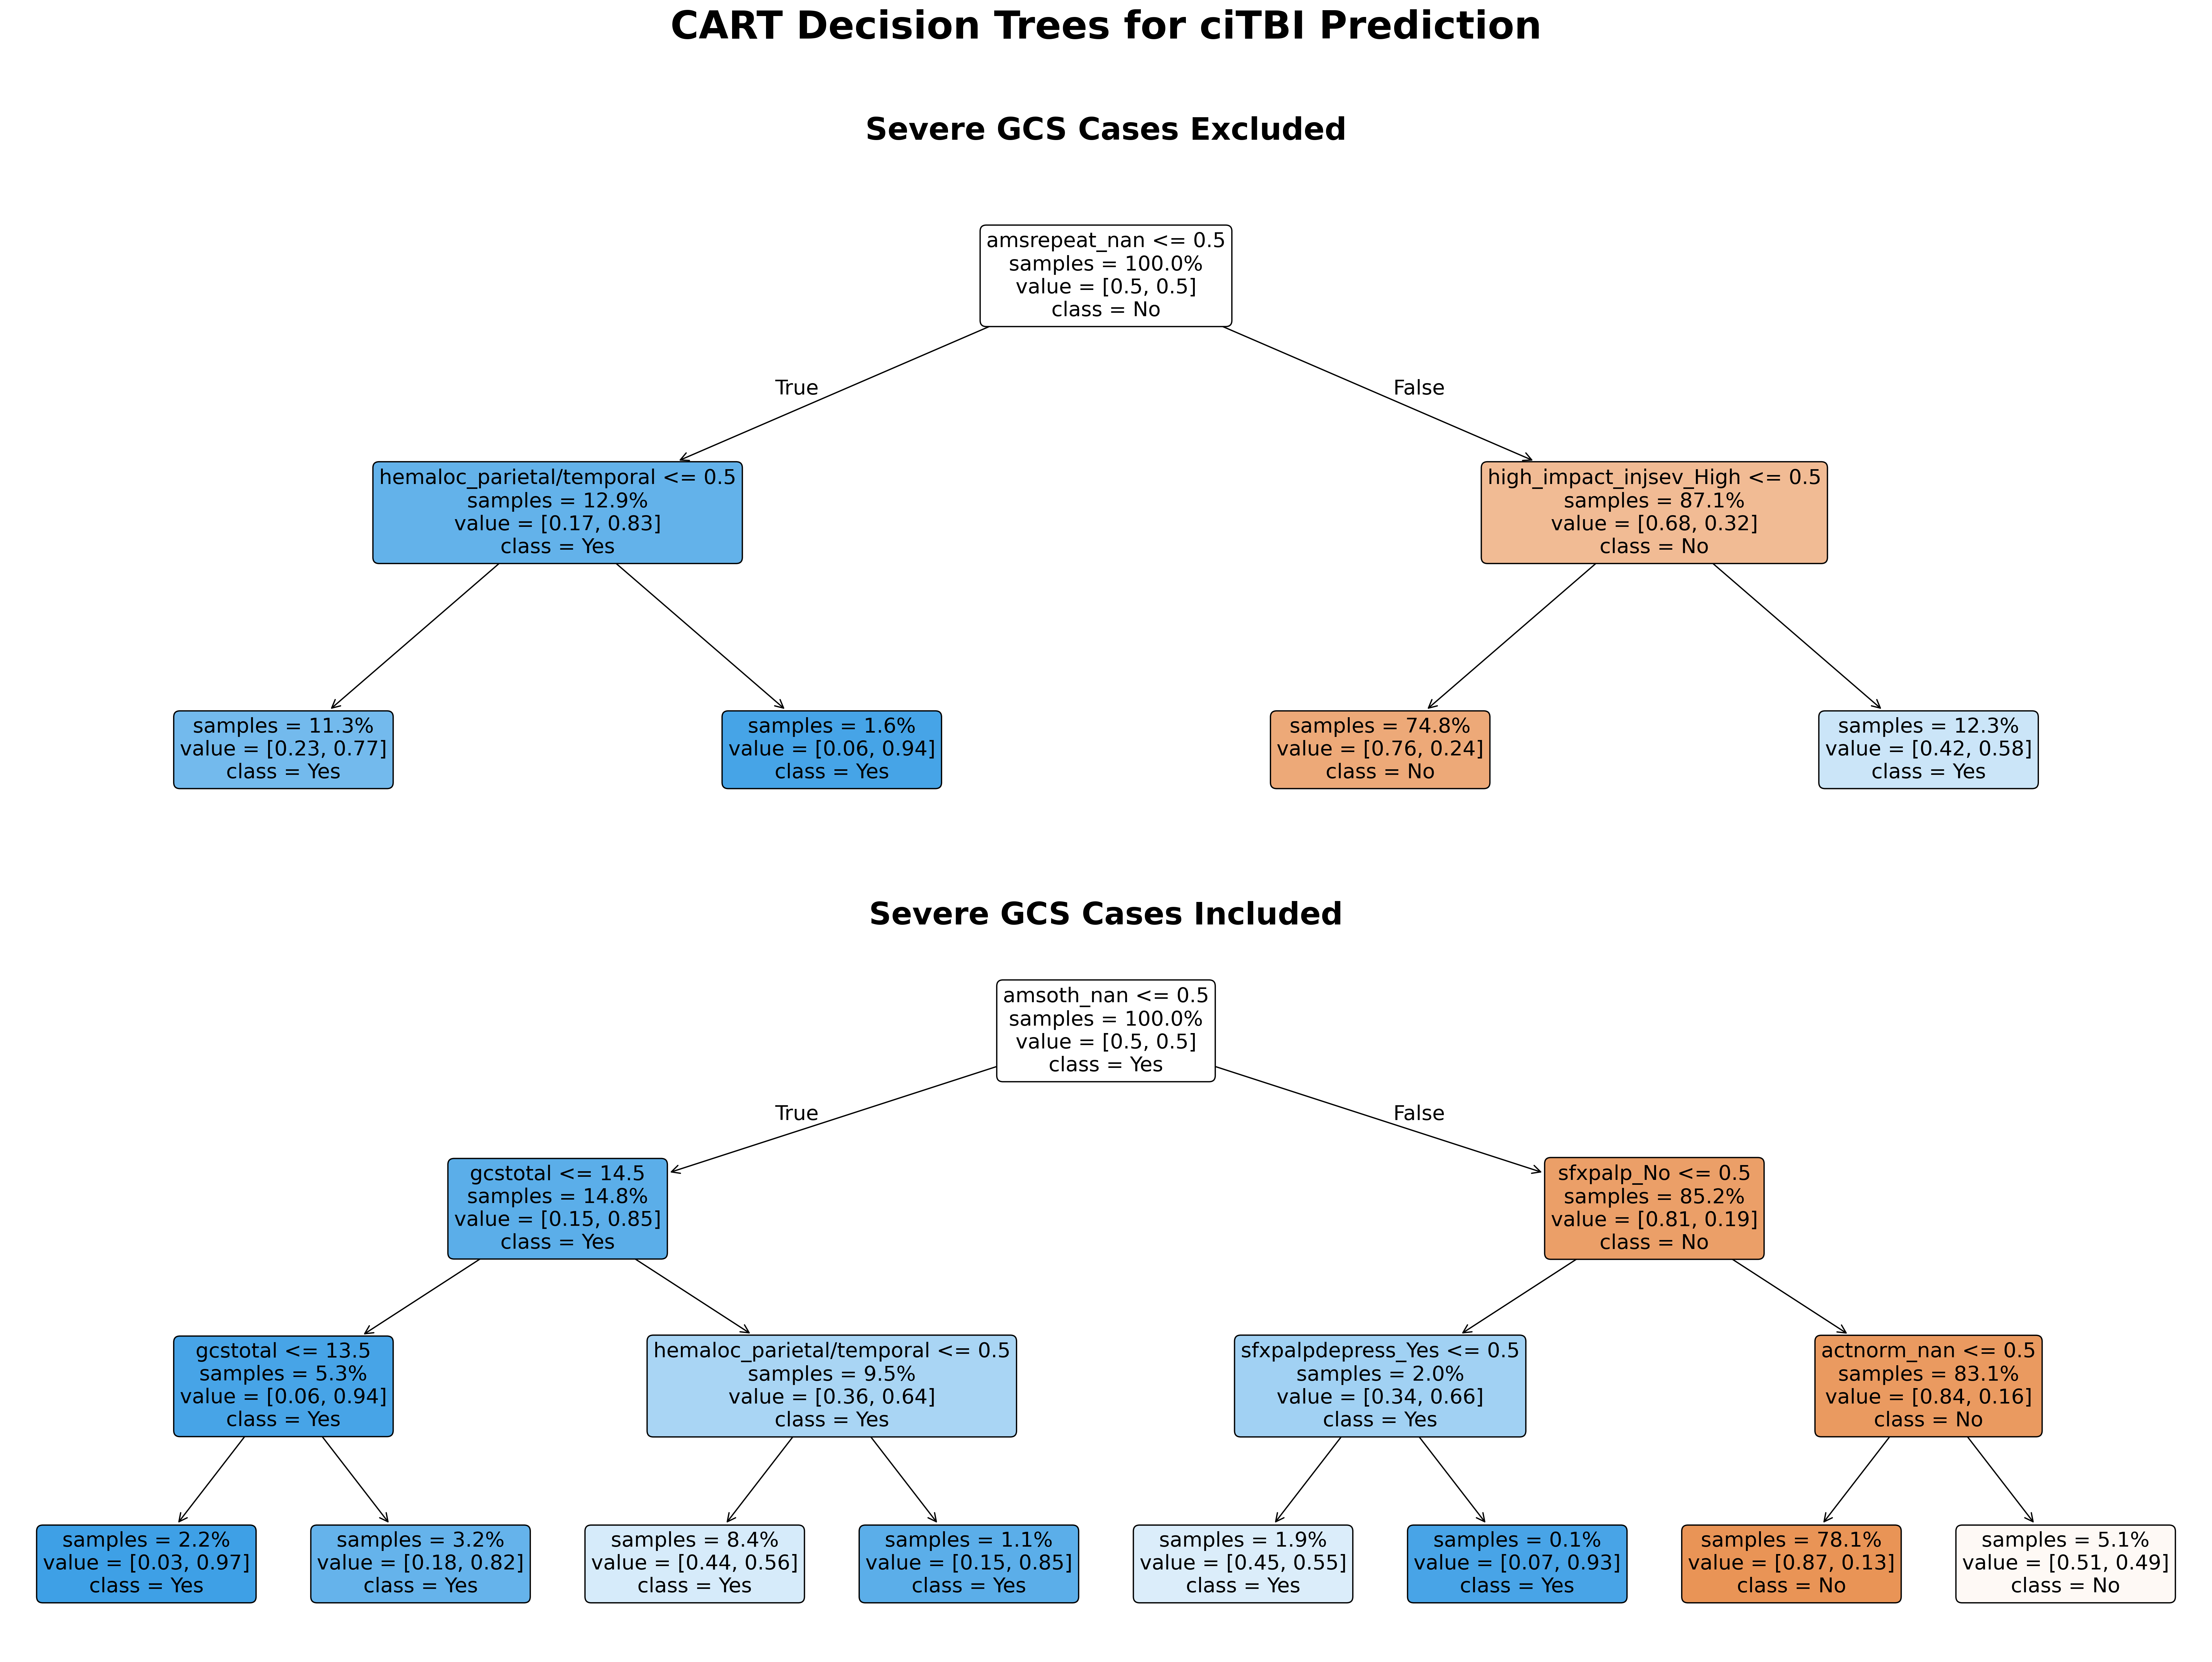
\includegraphics[width=0.9\linewidth]{../figs/cart_tree_comparison.png}
    \caption{CART schematics for both perturbations of data.}
    \label{fig:CART_comparison}
\end{figure}

The greatest change between the two perturbed datasets is therefore seen primarily in the model performance. Including severe cases seems to provide a better trained model but may be of less use to the clinician who is mostly concerned with he cases that are not as obvious to diagnose. 

\subsection{Discussion}
The CART model was chosen because of its interpretability and its structural similarity to the clinical decision rule developed by Kuppermann et al. A decision tree produces a sequence of simple, clinically interpretable splits that can be written down and followed directly by a clinician. This makes it particularly appropriate for a problem in which predictions may ultimately inform a diagnostic decision. Gradient boosting was chosen as a contrasting approach because it can represent substantially more complex relationships than a single tree and therefore provides a useful comparison between predictive performance and interpretability. Together, the two models allow us to ask whether increased model flexibility provides meaningful gains in prediction relative to the transparency of a simple decision rule.\\

The CART model is a simple and directly interpretable form: its predictions can be traced through the individual splits of the tree to the resulting classification. The gradient boosting model is considerably less interpretable because its predictions result from the combined contributions of many sequentially fitted trees. For this model, we rely primarily on variable importance to understand which clinical observations contribute most to prediction, while recognizing that importance measures do not describe the specific decision process for an individual patient. Thus, although variable importance provides some insight into how the model uses the data, it does not offer the same level of clinical transparency as the explicit decision rules produced by CART.


\section{Conclusion}\label{conclusion}

This paper examines the PECARN data through the PCS framework, focusing on how data-cleaning choices affect the downstream data science process. The data are messy: substantial missingness and complex hierarchical relationships bind clinical variables. We therefore centered the cleaning process on the clinical context in which the data were collected, distinguishing between information that could be logically reconstructed and decisions that required domain-informed judgment. The reality check suggests that the cleaned data largely reflect clinically plausible patterns. These data represent a snapshot of an extremely volatile emergency-room environment, and missing or inconsistent observations may reflect circumstances that are not captured in the dataset.\\

The modeling portion of the analysis demonstrates how these data-cleaning decisions propagate into the algorithmic realm of the PCS framework. CART provides a simple and interpretable representation of the clinical decision process, while gradient boosting provides a more flexible but less interpretable alternative. Our findings suggest some reason to reconsider the strict two-year age cutoff and raise questions about how severe GCS cases should be handled. Importantly, these conclusions depend on how the underlying data are represented, reinforcing that model interpretation cannot be separated from the cleaning and preprocessing decisions that precede it.\\

This analysis highlights the value of collecting information that better captures the circumstances surrounding clinical observations, particularly when values are missing or appear inconsistent. The size of the PECARN dataset made comprehensive manual inspection impractical, increasing our reliance on systematic cleaning rules and visualization. At the same time, the large sample allowed us to examine stability across groups and perturbations of the cleaning process. The PCS perspective demonstrates that the data science life-cycle extends beyond model selection, understanding how clinical reality becomes data allows for better informed judgment calls in the modeling process. 


\section{Academic honesty statement}\label{academic-honesty-statement}

The work in this report is the product of original thought. I have, to the best of my ability, cited all sources of information which are not original to ensure credit is give where credit is due. The honest of this statement, and the importance of honesty in academic research, is imperative if we are to uphold the objective truths of science upon which we base our decisions, improve lives, and strive for human excellence. In a where answers are so easy to come by and AI has automateand will automate many intelectual tasks, it falls on all of us to struggle with learning in order to preserve our humanity. 

\section{Collaborators}
I would like to acknowledge the conversations I had with June Park, Prithika Roy, Brileigh Cates, and Peter Zakariya that helped inspire this paper. The extent of collaboration was purely discussion; all code, reasoning, and evaluation is original or properly attributed to its source. 

\section{AI Statement}
AI was utilized for coding assistance (CoPilot) and LaTeX formatting (Gemini). All code was drafted by hand and all analysis and writing has been produced by the author of this paper without AI assistance.

\printbibliography

\end{document}

